\documentclass[10pt,letterpaper]{article}

% Compile from this directory with: latexmk -pdf main.tex
% Typography follows the essential ICLR conventions: Times text, a single
% 5.5-inch column, compact headings, and author--year references.
% Reference: https://github.com/ICLR/Master-Template
% No conference affiliation, review banner, or submission line numbering.
\usepackage[T1]{fontenc}
\usepackage[utf8]{inputenc}
\usepackage{times}
\usepackage[letterpaper,textwidth=5.5in,textheight=9in,top=0.9in]{geometry}
\usepackage{amsmath,amssymb,amsthm}
\usepackage{microtype}
\usepackage{booktabs,tabularx,array}
\usepackage{graphicx}
\graphicspath{{figures/}}
\usepackage{placeins}
\usepackage{algorithm}
\usepackage{algpseudocode}
\usepackage{needspace}
\usepackage{etoolbox}
\usepackage[round,authoryear]{natbib}
\usepackage[hidelinks,pdfusetitle]{hyperref}

\makeatletter
\renewcommand\normalsize{\@setfontsize\normalsize{10pt}{11pt}}
\renewcommand\small{\@setfontsize\small{9pt}{10pt}}
\renewcommand\section{\@startsection{section}{1}{\z@}
  {-2.0ex plus -.4ex minus -.2ex}{1.2ex plus .2ex}
  {\large\scshape\raggedright}}
\renewcommand\subsection{\@startsection{subsection}{2}{\z@}
  {-1.8ex plus -.4ex minus -.2ex}{.8ex plus .2ex}
  {\normalsize\scshape\raggedright}}
\renewcommand\paragraph{\@startsection{paragraph}{4}{\z@}
  {1.2ex plus .3ex minus .2ex}{-1em}{\normalsize\bfseries}}
\renewcommand\maketitle{%
  \begin{center}
    {\fontsize{17}{20}\selectfont\scshape\@title\par}
  \end{center}\vspace{.6em}}
\makeatother
\normalsize

\renewenvironment{abstract}
  {\begin{center}\scshape Abstract\end{center}\begin{quote}\small}
  {\end{quote}\vspace{.4em}}
\setlength{\parindent}{0pt}
\setlength{\parskip}{5pt plus 1pt minus 1pt}
\setlength{\abovedisplayskip}{6pt plus 1pt minus 1pt}
\setlength{\belowdisplayskip}{6pt plus 1pt minus 1pt}
\setlength{\abovedisplayshortskip}{3pt plus 1pt}
\setlength{\belowdisplayshortskip}{4pt plus 1pt}
\setlength{\textfloatsep}{8pt plus 1pt minus 1pt}
\setlength{\floatsep}{6pt plus 1pt minus 1pt}
\setlength{\intextsep}{5pt plus 1pt minus 1pt}
\setlength{\abovecaptionskip}{4pt}
\setlength{\belowcaptionskip}{1pt}
\setlength{\bibsep}{4pt plus 1pt}
\setcitestyle{citesep={;},aysep={,},yysep={;}}
\renewcommand{\bibsection}{\section*{References}}
\renewcommand{\topfraction}{.9}
\renewcommand{\textfraction}{.1}

% Keep prose paragraphs intact and keep headings with their opening text.
% A finite parfillskip discourages very short paragraph-ending lines.
\widowpenalty=10000
\clubpenalty=10000
\displaywidowpenalty=10000
\interlinepenalty=10000
\brokenpenalty=10000
\predisplaypenalty=10000
\postdisplaypenalty=10000
\setlength{\parfillskip}{0pt plus .72\linewidth}
\setlength{\emergencystretch}{1em}
\raggedbottom
\pretocmd{\section}{\Needspace{5\baselineskip}}{}{}
\pretocmd{\subsection}{\Needspace{4\baselineskip}}{}{}
\pretocmd{\paragraph}{\Needspace{4\baselineskip}}{}{}
\AtBeginEnvironment{thebibliography}{%
  \small
  \interlinepenalty=10000
  \setlength{\parfillskip}{0pt plus 1fil}}

\newcommand{\States}{\mathcal{S}}
\newcommand{\Actions}{\mathcal{A}}
\newcommand{\Terminal}{\mathcal{Z}}
\newcommand{\Tactical}{\mathcal{C}}
\newcommand{\Book}{\mathcal{B}}
\newcommand{\Search}{\mathsf{S}}
\newcommand{\ind}{\mathbf{1}}
\newcommand{\chessmove}[1]{\mbox{\normalfont #1}}
\newsavebox{\deploymentimage}
\newlength{\deploymentheight}
% Match the image with natural prose. A small finite glue allowance balances
% the pair; it cannot hide a short text block behind a large paragraph gap.
\newcommand{\deploymentpair}[3]{%
  \sbox{\deploymentimage}{\includegraphics[width=.48\linewidth]{#1}}%
  \setlength{\deploymentheight}{\dimexpr\ht\deploymentimage+\dp\deploymentimage\relax}%
  \begin{minipage}[t]{.48\linewidth}
    \vspace{0pt}\usebox{\deploymentimage}
  \end{minipage}\hfill
  \begin{minipage}[t][\deploymentheight][s]{.48\linewidth}
    \vspace{0pt}%
    \setlength{\parfillskip}{0pt plus 1fil}%
    \setlength{\parskip}{5pt}%
    \setlength{\emergencystretch}{.5em}%
    #2\par
    \vskip 0pt plus 4pt
    #3\unskip\strut\par
    \vspace{0pt}%
  \end{minipage}%
}
\DeclareMathOperator*{\argmax}{arg\,max}
\newtheorem{proposition}{Proposition}
\newcolumntype{Y}{>{\raggedright\arraybackslash}X}

\title{Selective Adversarial Search for Chess\\under Time Constraints}
% Add verified author names and affiliations here when needed.
\author{}
\date{}

\begin{document}
\maketitle

\begin{abstract}
A chess engine must compare adversarial continuations within a limited time
budget. Its decisions depend on both the positions it examines and the values
assigned to its search frontier. We describe a classical search method that
combines negamax backups with alpha--beta pruning, a phase-dependent positional
evaluation, and tactical continuation at the nominal horizon. Iterative
deepening maintains a completed decision as search proceeds. Move ordering and
transposition reuse reduce repeated work, while bounded extensions and late move
reductions allocate depth according to tactical relevance. An opening book
provides a separate decision rule for covered early positions. We give a common
mathematical formulation of these components and identify the assumptions under
which pruning preserves a fixed-tree minimax value. A desktop deployment connects
this procedure to a live game through asynchronous search, clock-aware budgets,
and validation of returned actions. Annotated game states and an execution trace
illustrate the interaction between the search rules and the deployed agent.
\end{abstract}

\section{Introduction}
\label{sec:introduction}

Chess makes the cost of deliberation explicit. Every legal move permits a set of
opponent replies, each of which creates further choices. A useful decision
therefore requires an estimate of what both players can achieve along a
continuation. Exhaustive analysis becomes infeasible as the horizon grows, so a
practical engine must decide where to stop, how to value the resulting
positions, and which parts of the tree deserve additional computation.

The classical approach couples a search procedure with a positional evaluation
\citep{shannon1950}. Search exposes consequences that are difficult to recognize
from the current board alone. Evaluation supplies information about continuations
beyond the examined horizon. These components interact: an immediate material
gain may disappear after a recapture, and a forcing sequence may remain
unresolved when a uniform depth limit is reached. The choice of search frontier
is consequently part of the decision method.

\paragraph{Approach and scope.}
We study this interaction in a chess engine with fixed evaluation parameters and
a finite deliberation budget. The engine searches in the negamax form of
minimax. Alpha--beta bounds eliminate continuations that cannot affect an
ancestor's decision, and tactical search refines frontier positions. Depth is
allocated selectively through extensions and reductions. Search results also
inform move ordering and can be reused when the same position is encountered
again. Iterative deepening connects these mechanisms to a deadline by retaining
the action from the latest completed root search.

We formulate an integration of established techniques at the level of states,
values, search bounds, and resource allocation. The formulation specifies how
the positional evaluator interacts with the tactical frontier and identifies the
scope of the fixed-tree pruning guarantee. We then describe how this decision
procedure operates within a desktop game, including the transfer of game state,
interruption of search, and validation of a returned action. Captured positions
and worker messages make these interactions observable. Playing strength and
the benefit of individual search enhancements require separate evaluation.

\section{Related Work}
\label{sec:related}

\paragraph{Classical chess search.}
\citet{shannon1950} formulated computer chess around the combination of
look-ahead search and position evaluation. \citet{knuth1975} analyzed
alpha--beta pruning and the dependence of its cost on move ordering.
\citet{schaeffer1989} examined the history heuristic together with other
search enhancements, including transposition tables and killer moves. These
techniques provide the search foundation used here. Their interaction matters
because a promising move examined early can establish a bound that avoids
substantial work later in the same search.

\paragraph{Selective analysis and evaluation.}
The design of Deep Blue illustrates the importance of nonuniform search,
extensions, quiescence analysis, and structured chess knowledge
\citep{campbell2002}. These mechanisms address different sources of error:
evaluation estimates positional value, while additional search resolves
concrete tactical consequences. Our formulation uses a compact collection of
material, placement, pawn, king, and center terms, together with a bounded
selective search. The description concerns the roles of these components and
the decision rules that connect them.

\paragraph{Learning and search.}
AlphaZero combines self-play learning with neural policy and value functions and
Monte-Carlo tree search \citep{silver2018}. \citet{grill2020} interpret its
action-selection mechanism through regularized policy optimization. These works
show how a search procedure can operate with learned estimates and action
preferences. In the present engine, evaluation parameters are prescribed,
action preferences come from search statistics and chess features, and values
are propagated by adversarial negamax backups. The common issue is how a
limited search budget is allocated across candidate continuations.

\section{Problem Formulation}
\label{sec:problem}

\paragraph{Game model.}
Let $\States$ be the set of legal game states. A state $s$ contains the board,
the player to move $c(s)$, castling and en-passant rights, and the history needed
to determine draw conditions. We write $\bar c$ for the opponent of player $c$,
$\Actions(s)$ for the legal actions, and $T(s,a)$ for the deterministic successor.
Each transition changes the player to move. A \emph{ply} is one such transition.

Let $\Terminal\subset\States$ denote terminal states. Search assigns a draw
value of zero and a checkmate value from the perspective of the player to move:
\begin{equation}
  \tau(s,\ell)=
  \begin{cases}
    -M+\ell, & \text{if the player to move is checkmated},\\
    0,       & \text{if the search recognizes a draw},
  \end{cases}
  \qquad s\in\Terminal,
  \label{eq:terminal}
\end{equation}
where $\ell$ is the distance from the current root. For the static evaluator
$E_\theta$ defined in Section~\ref{sec:evaluation}, choose
$M-L_{\max}>\sup_{s\notin\Terminal}|E_\theta(s)|$ so that mate values dominate
heuristic scores. Negating the terminal value along a path gives a preference
for an earlier forced win and a later forced loss. Draw detection covers
stalemate, insufficient material, repetition, and the move-count rule adopted
by the engine.

\paragraph{Decision objective.}
For a nonterminal state, the decision procedure receives a time allowance $B$
and a maximum nominal depth $d_{\max}$. Its output is a legal action
$\hat a\in\Actions(s)$. The underlying game objective is the zero-sum terminal
outcome. Within the available budget, the engine approximates that objective
through a finite tree whose frontier is scored by a heuristic evaluator.
An evaluation score expresses relative positional preference; it carries
no calibrated interpretation as a probability of winning.

\section{Search Framework}
\label{sec:method}

The decision procedure has three stages. It first checks whether an eligible
opening-book action is available. Otherwise, it performs root searches at
increasing nominal depths. Each search combines bounded adversarial backups
with positional evaluation and tactical continuation at the frontier.
Algorithm~\ref{alg:decision} gives the resulting budgeted decision rule.

\subsection{Positional Evaluation}
\label{sec:evaluation}

For player $c$, let $F_\theta(s,c)$ measure the strength of that player's
position. The parameter collection $\theta$ contains fixed piece values,
positional tables, and feature weights. We decompose the score as
\begin{equation}
  F_\theta(s,c)
  = M_c(s)+L_c(s)+P_c(s)+K_c(s)+C_c(s)+W_c(s).
  \label{eq:components}
\end{equation}
The terms represent material, piece placement, pawn structure, king safety,
central control, and endgame conversion. All use a common score scale.
Table~\ref{tab:evaluation} summarizes the information they encode.

The parameters are specified before play and shared across searched positions.
Position-dependent features, including the phase variables, are recomputed as
moves change the board. Search statistics alter exploration order without
updating $\theta$. The resulting score expresses the current arrangement under
a fixed set of positional preferences.

\begin{table}[H]
  \centering
  \small
  \caption{Components of the positional evaluator. Parameters specify the
  relative strength of each feature within the shared score scale.}
  \label{tab:evaluation}
  \begin{tabularx}{\linewidth}{@{}lY@{}}
    \toprule
    Term & Chess information \\
    \midrule
    $M_c$ & Weighted counts of pawns, knights, bishops, rooks, and queens. \\
    $L_c$ & Piece-specific square preferences, with phase-dependent tables
            for pawns and kings. \\
    $P_c$ & Advancement of passed pawns and penalties for isolated pawns. \\
    $K_c$ & Pawn cover and exposed files near the king, weighted by game phase
            and opposing heavy pieces. \\
    $C_c$ & Occupation and attacks on central squares and the surrounding ring. \\
    $W_c$ & King coordination and opposing king displacement during
            conversion of a material lead. \\
    \bottomrule
  \end{tabularx}
\end{table}

\paragraph{Material and placement.}
Write $\mathcal{P}_c(s)$ for the pieces of player $c$, and let $t(p)$ and $q(p)$
denote a piece's type and square. Material and placement take the form
\begin{equation}
  M_c(s)=\sum_{p\in\mathcal{P}_c(s)}v_{t(p)},
  \qquad
  L_c(s)=\sum_{p\in\mathcal{P}_c(s)}
              b_{t(p)}\bigl(q(p),c;\phi_c(s)\bigr).
  \label{eq:material}
\end{equation}
The king's material weight is zero because checkmate is handled by
Equation~\eqref{eq:terminal}. Square tables use a consistent orientation for
both colors.

\paragraph{Phase and structure.}
The phase variable is determined by the opponent's remaining material outside
pawns and kings. If that material is $m_{\bar c}^{\mathrm{np}}(s)$ and the
reference scale is $m_0>0$, then
\begin{equation}
  \phi_c(s)=\max\left\{0,1-\frac{m_{\bar c}^{\mathrm{np}}(s)}{m_0}\right\},
  \qquad
  b_t(q,c;\phi)=(1-\phi)b_t^{\mathrm{early}}(q,c)
                        +\phi b_t^{\mathrm{late}}(q,c).
  \label{eq:phase}
\end{equation}
Nonnegative material gives $\phi_c(s)\in[0,1]$. For piece types with a single
table, the two endpoint tables coincide. This construction allows pawn
advancement and king activity to gain value as the opposing force is reduced.
The two players can have different phase values in an asymmetric position.

The remaining terms express structural features of the current board. A passed
pawn has no opposing pawn ahead on its own or an adjacent file; its bonus grows
as promotion approaches. Isolated pawns lack a friendly pawn on an adjacent
file. King safety penalizes missing pawn cover and nearby files exposed to
heavy pieces, with reduced weight in the endgame. Central control rewards both
occupation and attacks. The conversion term becomes active with a sufficient
material lead and favors coordinated king activity against an opposing king
away from the center.

\paragraph{Evaluation perspective.}
The static value uses the perspective required by negamax:
\begin{equation}
  E_\theta(s)
  =F_\theta(s,c(s))-F_\theta(s,\overline{c(s)})
     -\kappa\,\ind\{c(s)\text{ is in check}\},
  \label{eq:evaluation}
\end{equation}
where $\kappa\ge0$ is the check penalty.

\subsection{Adversarial Backups and Search Bounds}
\label{sec:backups}

We first define a reference search with a fixed nominal horizon. Let
$Q_\theta(s,\ell)$ be the tactical frontier value specified in
Section~\ref{sec:quiescence}. With a maximum path length $L_{\max}$, the reference
value is
\begin{equation}
  V_d(s,\ell)=
  \begin{cases}
    \tau(s,\ell), & s\in\Terminal,\\
    E_\theta(s), & \ell\ge L_{\max},\\
    Q_\theta(s,\ell), & d\le0,\\
    \displaystyle\max_{a\in\Actions(s)}
       \bigl[-V_{d-1}(T(s,a),\ell+1)\bigr], & \text{otherwise}.
  \end{cases}
  \label{eq:negamax}
\end{equation}
The sign change accounts for alternating players in a zero-sum game.
At a completed root search with $d\ge1$, the corresponding decision is
\begin{equation}
  a_d\in\argmax_{a\in\Actions(s)}
      \bigl[-V_{d-1}(T(s,a),1)\bigr].
  \label{eq:root}
\end{equation}
This maximization assumes that each opponent reply is selected to maximize the
opponent's value. It therefore evaluates a candidate through the strongest
response found within the examined tree.

\paragraph{Alpha--beta bounds.}
Alpha--beta search evaluates this recursion with a window $[\alpha,\beta)$.
The lower threshold $\alpha$ tracks the best established alternative; the upper
threshold $\beta$ is inherited from an ancestor's alternatives. If action $a_i$
has returned value $q_i$, the update is
\begin{equation}
  \alpha_{i+1}=\max\{\alpha_i,q_i\},
  \qquad
  \alpha_{i+1}\ge\beta
    \ \Longrightarrow\ \text{stop expanding the remaining actions}.
  \label{eq:cutoff}
\end{equation}
A recursive negamax call uses the reversed window $[-\beta,-\alpha_i)$.
A cutoff establishes a sufficient bound for an ancestor's choice. The returned
quantity may therefore be a bound on a node's value.

\subsection{Tactical Continuation at the Frontier}
\label{sec:quiescence}

A depth limit can interrupt an exchange immediately after one side captures a
piece. Static evaluation at that point can assign value to a gain that the
opponent can immediately recover. Quiescence search extends the frontier
through a restricted set of tactical actions.

\paragraph{Tactical actions and backups.}
For a nonterminal state, define
\begin{equation}
  \Tactical(s)=
  \begin{cases}
    \Actions(s), & c(s)\text{ is in check},\\
    \{a\in\Actions(s):a\text{ captures or promotes}\}, & \text{otherwise}.
  \end{cases}
  \label{eq:tactical-actions}
\end{equation}
Let $g(s)=-\infty$ when the player to move is in check, and
$g(s)=E_\theta(s)$ otherwise. The unpruned tactical target is
\begin{equation}
  Q_\theta(s,\ell)=
  \begin{cases}
    \tau(s,\ell), & s\in\Terminal,\\
    E_\theta(s), & \ell\ge L_{\max},\\
    \displaystyle\max\left\{g(s),
      \max_{a\in\Tactical(s)}
           [-Q_\theta(T(s,a),\ell+1)]\right\}, & \text{otherwise}.
  \end{cases}
  \label{eq:quiescence}
\end{equation}
We use $\max\varnothing=-\infty$. Away from check, the static score serves as
the \emph{stand-pat} candidate. In check, every legal evasion is considered and
the stand-pat candidate is disabled. The path cap ensures termination even
when tactical continuations include long sequences of checks.

Alpha--beta bounds also apply within this tactical tree. The stand-pat
candidate is a heuristic assumption about the value of stopping local tactical
analysis. Positions involving zugzwang can violate that assumption. Tactical
continuation resolves only the classes of moves in
Equation~\eqref{eq:tactical-actions}; quiet threats can remain beyond its
frontier.

\subsection{Selective Depth Allocation}
\label{sec:selective}

Uniform depth assigns the same remaining horizon to actions with very different
tactical consequences. The engine modifies this allocation in two ways.
An extension preserves additional depth for checks and advanced pawn moves.
A reduction first examines eligible late quiet moves at a shorter horizon.
Eligibility excludes captures, promotions, positions already in check, and
moves receiving an extension.

\paragraph{Depth allocation.}
For an action $a_i$ in search order, write
\begin{equation}
  d_i=d-1+e(s,a_i),
  \qquad
  d_i^{\mathrm{test}}=d_i-r(s,a_i,d,i),
  \label{eq:selective-depth}
\end{equation}
where $e\ge0$ and $r\ge0$ are bounded integer adjustments.
A pathwise extension allowance limits accumulated extensions, and $L_{\max}$
bounds the total path length.

\paragraph{Reduced-depth probes.}
Let $\Search(s,d,\alpha,\beta)$ denote the practical bounded search, with root
distance and path allowances implicit. For an eligible reduced action with
successor $s_i=T(s,a_i)$, a narrow-window probe computes
\begin{equation}
  \widetilde q_i
  =-\Search\bigl(s_i,d_i^{\mathrm{test}},
                 -\alpha_i-\delta,-\alpha_i\bigr),
  \label{eq:probe}
\end{equation}
where $\delta>0$ is the score resolution. If
$\widetilde q_i>\alpha_i$, the action is searched again at depth $d_i$ with the
full current window. Other actions are searched directly at depth $d_i$.

The probe asks whether the action can improve the incumbent value. Its shorter
horizon provides a low-cost test, but can underestimate a continuation whose
benefit appears later. Re-search recovers some promising actions; a reduced
action that fails the test receives no deeper verification. The practical
search can consequently select a different action from the fixed-horizon rule
in Equation~\eqref{eq:root}.

\subsection{Ordering and Transposition Reuse}
\label{sec:reuse}

Move ordering uses information from the current position and previous search
work. A stored best move receives priority, captures are ranked using the
values of the victim and attacker, and promotions receive a tactical preference.
Quiet actions are also ranked through killer moves and a history score. Killer
moves record quiet actions that caused a cutoff at the same root distance.
The history score accumulates credit for quiet actions that caused cutoffs,
with larger credit for greater search depth \citep{schaeffer1989}. These
statistics are exploration preferences within the current decision process.

\paragraph{Cached bounds.}
A transposition record stores a position key, the searched depth, the returned
score, its bound type, and a preferred action. Under a compatible horizon and
search context, a record with score $v$ has one of three meanings:
\begin{equation}
  V=v\quad(\text{exact}),\qquad
  V\ge v\quad(\text{lower bound}),\qquad
  V\le v\quad(\text{upper bound}).
  \label{eq:bounds}
\end{equation}
An eligible exact record supplies a value directly. A lower bound at least
$\beta$, or an upper bound at most $\alpha$, suffices to end the current query.
The stored action can guide ordering even when the value is ineligible.

The engine uses a compact key for the board position and move-count state,
filters reuse at nodes with detected repetition, and accepts records whose
stored depth meets the current depth request. Mate values are normalized for
root distance before reuse. These rules support practical reuse; compatibility
with the full history and selective-search context remains a separate
requirement. In particular, an entry from a deeper horizon supplies information
from a different search tree.

\subsection{Opening Knowledge and Budgeted Decisions}
\label{sec:budget}

The opening book maps covered early positions to legal candidate actions with
nonnegative weights $w(s,a)$. For a relative threshold $\eta\in(0,1]$, define
\begin{equation}
  \Book_\eta(s)=
  \left\{a\in\Book(s):
    w(s,a)\ge\eta\max_{b\in\Book(s)}w(s,b)\right\}.
  \label{eq:book}
\end{equation}
When this set is nonempty and the state lies within the permitted opening
prefix, an action is sampled uniformly from $\Book_\eta(s)$. For other
nonterminal states, the engine invokes search. The book weights are external
inputs to this rule.

\paragraph{Iterative deepening.}
Search proceeds at nominal depths $1,2,\ldots,d_{\max}$. Let $t_d$ be the elapsed
time when iteration $d$ completes and $\hat a_d$ its returned action. The
budgeted decision is
\begin{equation}
  \hat a_B=\hat a_{d^\star},
  \qquad
  d^\star=\max\{d\le d_{\max}:t_d\le B\},
  \label{eq:budget}
\end{equation}
whenever at least one iteration completes. A legal fallback is retained for
earlier interruption. The engine can also stop after finding a mate-valued
result. A partially explored iteration leaves the last completed decision
available.

\begin{algorithm}[!ht]
  \caption{Budgeted chess decision}
  \label{alg:decision}
  \begin{algorithmic}[1]
    \Require Nonterminal state $s$, time allowance $B$, depth limit $d_{\max}$
    \State If $\Book_\eta(s)$ is eligible, return a uniform sample from it
    \State Retain a legal fallback action $\hat a\in\Actions(s)$
    \For{$d=1,\ldots,d_{\max}$}
      \State Run selective search at depth $d$ within the remaining time allowance
      \State If interrupted, stop and retain the previous action
      \State Retain its returned action as $\hat a$
      \State Stop if a mate-valued result is found
    \EndFor
    \State \Return $\hat a$
  \end{algorithmic}
\end{algorithm}

An interrupted pass may contain fully evaluated subtrees. Their cached bounds
remain subject to the compatibility requirements in Section~\ref{sec:reuse}.
Updating such a record leaves the retained root action unchanged; the action
is replaced only after a successful iteration. This preserves a completed
decision while allowing reusable local work to accumulate.

\section{Search Properties}
\label{sec:properties}

The value-preserving property of alpha--beta concerns a fixed search tree
with compatible leaf values and reused bounds \citep{knuth1975}.

\begin{proposition}[Fixed-tree pruning]
Consider a finite alternating game tree with fixed leaf scores from the
player-to-move perspective. Alpha--beta search with a full root window
returns its exhaustive negamax value, provided every reused bound is valid
for the queried subtree. Move ordering can change the amount of work and the
choice among tied actions.
\end{proposition}

\begin{proof}
Negamax propagates each child value with a sign change. After any prefix of
the action list, $\alpha$ is at least the largest established candidate.
When a candidate reaches $\beta$, an ancestor already has an alternative
that makes the unexamined remainder irrelevant to its maximizing choice.
Pruning that remainder preserves the ancestor's backed-up value.
Applying this argument inductively from the leaves to the full-window root
proves the claim.
\end{proof}

\paragraph{Scope of the guarantee.}
The proposition applies to a tactical frontier treated as part of the fixed
tree. It also applies to extensions whose allocation is fixed in advance.
Late move reductions make depth depend on ordering and intermediate bounds,
and cross-depth transposition reuse can change the evaluated horizon.
Equation~\eqref{eq:budget} therefore returns the outcome of a completed
\emph{selective} iteration.

\paragraph{Computational cost.}
For a regular tree with branching factor $b$ and depth $D$, exhaustive search
examines $b^D$ leaves. With ideal move ordering and even $D$, alpha--beta needs
$2b^{D/2}-1$ leaves in the classical best case \citep{knuth1975}.
The worst-case order remains exponential. Extensions and tactical search
increase the effective depth; reductions decrease work selectively.
With at most $H$ transposition records, depth-first traversal stores
$O(bD+H)$ move and cache information, excluding the input game history.
Wall-clock cost additionally depends on legal-move generation and evaluation.

\FloatBarrier
\section{Deployment}
\label{sec:deployment}

The engine is deployed as the computer player in a local desktop chess
application. The interface maintains the live game, while a separate process
executes Algorithm~\ref{alg:decision}. This arrangement connects a potentially
long search to an interactive board and a running clock. The examples below
were captured from the application launched through \texttt{game.py}; arrows,
numbered pointers, and the trace plot are explanatory overlays.

\subsection{From a Live Position to a Committed Action}

\paragraph{State transfer.}
At the start of a computer turn, the application submits a snapshot of the
position and its move history to the search process. The worker reconstructs
the search state, including the history used for draw detection. Search then
operates on that snapshot while the interface continues to handle events.
Figure~\ref{fig:interface} identifies the information that connects the live
game to this decision: legal actions, remaining time, move history, and a
positional estimate.

\begin{figure}[!ht]
  \centering
  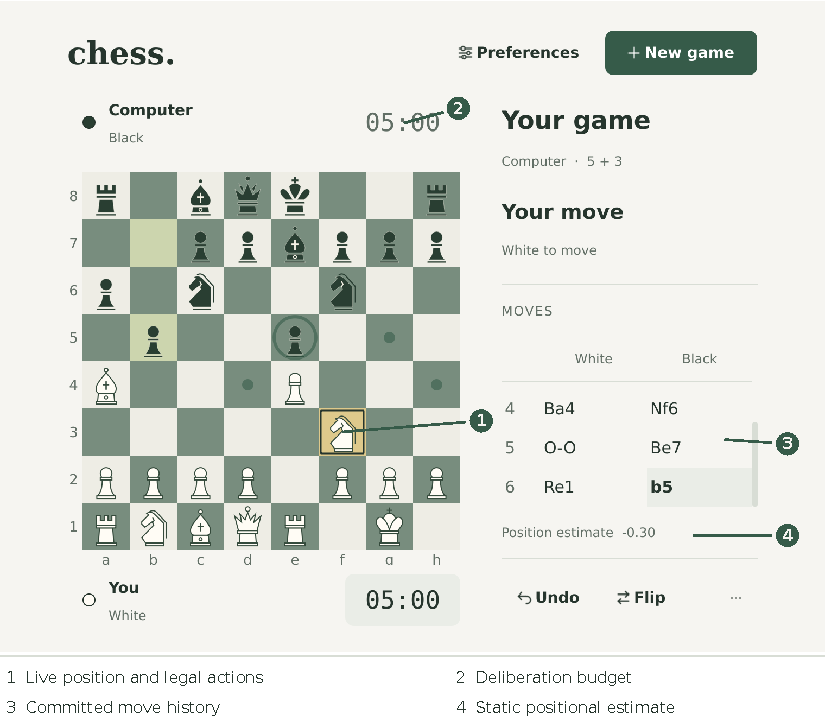
\includegraphics[width=\linewidth]{deployment-interface.pdf}
  \caption{The deployed chess interface, annotated to connect visible game
  information to the search framework. The selected knight exposes legal
  actions; clocks constrain deliberation; committed moves preserve game
  history. The optional position estimate displays the static evaluator from
  White's perspective, in pawn units. It is recomputed for the visible board.}
  \label{fig:interface}
\end{figure}

\begin{figure}[!ht]
  \centering
  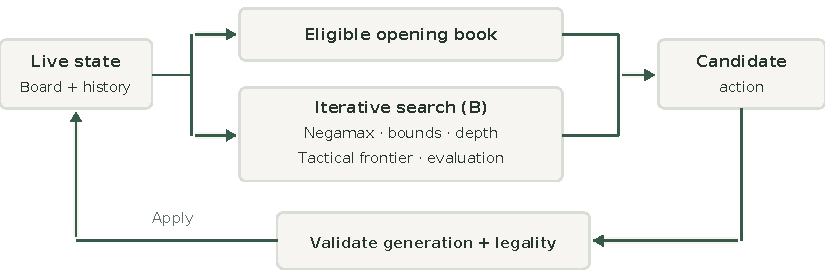
\includegraphics[width=\linewidth]{deployment-loop.pdf}
  \caption{The deployed decision loop. A state snapshot invokes either the
  eligible opening rule or budgeted search. Both paths return an action through
  the same validation step before the live game advances. The search block
  combines the mechanisms formalized in Section~\ref{sec:method}.}
  \label{fig:loop}
\end{figure}

\paragraph{Action validation.}
An interruption caused by a new game, a loaded position, or an undo invalidates
the outstanding search. Each request belongs to a generation of the live game;
a returned result is accepted only if that generation is still current. The
application also checks that the game remains active and the action is legal
before updating the board and clock. These checks keep a delayed response from
being applied to a changed position. Completed search iterations can update the
retained search result without changing the live board.
Figure~\ref{fig:loop} summarizes this separation between computing a candidate
and applying it to the game.

\paragraph{Clock-aware deliberation.}
Let $B_{\mathrm{cap}}$ be the configured allowance per move and
$B_{\mathrm{clock}}(s)$ the allowance derived from remaining time and increment.
For a timed game, the worker receives
\begin{equation}
  B(s)=\min\{B_{\mathrm{cap}},B_{\mathrm{clock}}(s)\}.
  \label{eq:deployed-budget}
\end{equation}
The clock allocation reserves time for future turns and execution overhead.
The resulting allowance controls the iterative decision rule in
Equation~\eqref{eq:budget}. Deadline and cancellation checks interrupt the
current traversal; the latest completed action remains available for return.
Process communication and interface updates occur outside the measured search
interval.

Figure~\ref{fig:iterations} shows this rule during a captured computer turn.
The fifth iteration completed at $1.282$\,s. Search continued until the
$1.800$\,s allowance was reached, and the returned action remained the
fifth iteration's \chessmove{dxc6}. The trace records nominal depth: extensions,
reductions, and tactical continuation can produce paths of different lengths
within an iteration. Its timestamps describe this execution on the host machine.

\begin{figure}[!ht]
  \centering
  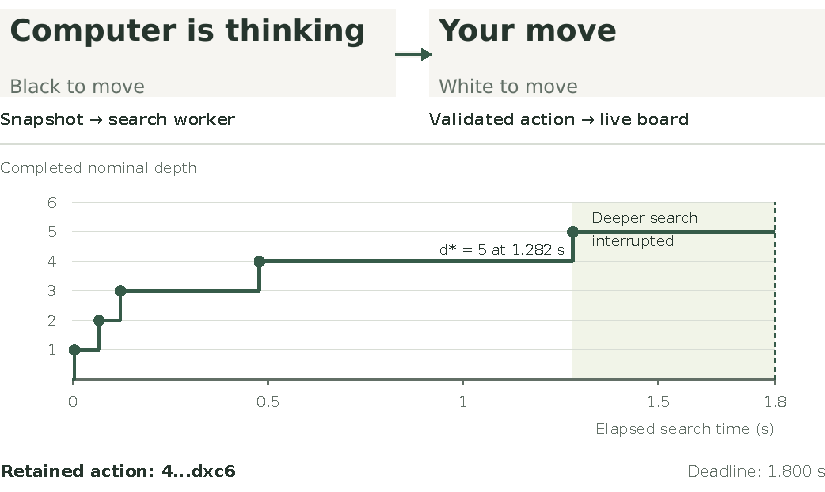
\includegraphics[width=\linewidth]{deployment-iterations.pdf}
  \caption{A captured search with the opening book disabled. Interface excerpts
  show the transition from computation to the human turn. The plot reconstructs
  completed iterations from worker messages, illustrating
  Equation~\eqref{eq:budget}. The shaded interval contains unfinished deeper
  search. Each completed iteration selected \chessmove{dxc6}, the action
  subsequently applied to the live game.}
  \label{fig:iterations}
\end{figure}

\FloatBarrier
Across the completed iterations, \chessmove{dxc6} remains the selected action
while its backed-up score changes from $-1.79$ to $-0.60$ pawn units. These
scores use Black's perspective at the search root and summarize different
examined continuations. The worker reports $12{,}000$ node visits at completion
of the fifth iteration and $17{,}394$ at interruption. The additional local
analysis leaves the completed root decision available, as required by
Algorithm~\ref{alg:decision}. The optional board estimate in Figure~\ref{fig:interface}
uses the current position and White's perspective, following the static
evaluation in Equation~\eqref{eq:evaluation}.

\subsection{Search Mechanisms in Play}

\begin{figure}[H]
  \deploymentpair{deployment-opening.pdf}{%
    \paragraph{Opening knowledge.}
    After the human plays \chessmove{e4}, the covered position invokes the book
    rule in Equation~\eqref{eq:book}. In this execution, the eligible set
    contains only \chessmove{c5}, so the computer selects that action directly.
    The arrow traces c7--c5. Book weights
    determine eligibility through the relative threshold; sampling is uniform
    over the surviving actions. Each eligible action has probability
    $1/|\Book_\eta(s)|$ at the covered state. At other covered positions, several entries
    may survive the threshold, so repeated games can
    \mbox{select different opening continuations.}
  }{%
    Book selection supplies an action without a completed root iteration or
    a backed-up search value. When the permitted prefix ends or no eligible
    entry exists, the worker invokes iterative deepening. The returned
    candidate passes the shared validation step in Figure~\ref{fig:loop};
    acceptance updates the board and
    \mbox{starts the next player's clock.}
  }
  \caption{An opening-book decision after \chessmove{1. e4}. The overlay traces
  c7--c5 on the live board. Book and search actions undergo the same validation
  before application.}
  \label{fig:opening}
\end{figure}

\Needspace{28\baselineskip}
\paragraph{An unsettled tactical frontier.}
Figure~\ref{fig:tactics} follows a human capture and the computer's reply in
the position used for Figure~\ref{fig:iterations}. After \chessmove{Bxc6}, White
has temporarily gained a knight. The reply \chessmove{dxc6} removes the capturing
bishop, leaving the material difference close to its initial value. A frontier
placed between these two actions would expose an incomplete exchange to static
evaluation. Equation~\eqref{eq:quiescence} addresses this situation by retaining
legal captures in the tactical action set; a search reaching the intermediate
position at its nominal horizon can therefore examine the recapture. At this
intermediate position Black is not in check. Its static score remains a
stand-pat candidate, and \chessmove{dxc6} belongs to $\Tactical(s)$. The tactical
backup compares the static value with the negated successor value of each
retained action.

\begin{figure}[H]
  \centering
  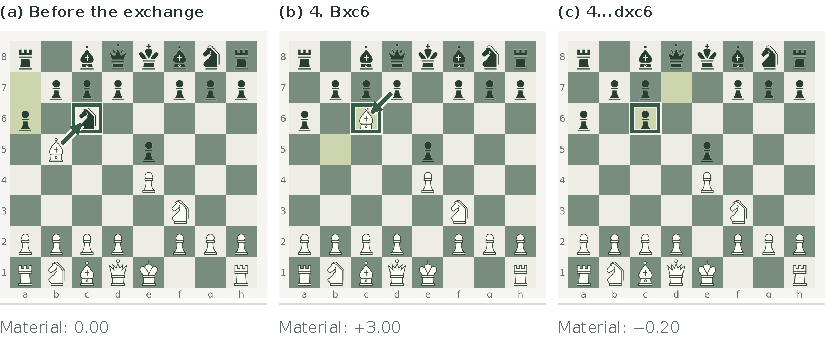
\includegraphics[width=\linewidth]{deployment-tactics.pdf}
  \caption{A captured exchange after \chessmove{1. e4 e5 2. Nf3 Nc6 3. Bb5 a6}.
  Arrows mark the human's \chessmove{4. Bxc6} and the engine's
  \chessmove{4...dxc6}. Outlines follow the exchange square. Material differences
  are shown from White's perspective in pawn units using the engine's piece
  weights; they exclude positional terms. The sequence illustrates the
  frontier issue addressed by tactical continuation.}
  \label{fig:tactics}
\end{figure}

\begin{figure}[H]
  \deploymentpair{deployment-endgame.pdf}{%
    \paragraph{Phase-dependent evaluation.}
    With only kings and White's three pawns present, both phase variables in
    Equation~\eqref{eq:phase} equal one. The late king table is fully active,
    and White's material lead activates the conversion term $W_c$. The engine
    completes a depth-three search and plays \chessmove{Kd4}, leaving all three
    pawns in place. The arrow identifies the king's advance on a board
    oriented toward the human playing Black.
  }{%
    At this transition, material and pawn structure remain unchanged, while
    king placement, central control, and conversion features change. Deeper
    continuations also examine pawn advances and opposing king replies. The
    phase and feature values are recomputed along those paths and combined
    through negamax backups. The selected king move connects these late
    positional preferences to a choice evaluated
    \mbox{through the opponent's replies.}
  }
  \caption{King activity in a captured endgame decision. White moves from c3
  to d4 while preserving its three pawns. The overlay identifies the action
  evaluated under the late-game phase; the position illustrates the operating
  context of the phase and conversion terms.}
  \label{fig:endgame}
\end{figure}

Together, these cases make three choices in Algorithm~\ref{alg:decision}
visible: selecting a covered opening action, resolving a tactical sequence,
and searching with phase-dependent frontier values. They document the
execution of the integrated engine. The contribution of each component to
move quality remains a question for controlled comparisons at matched budgets.

\FloatBarrier

\section{Discussion and Limitations}
\label{sec:limitations}

The decision procedure has three main approximation limits. First, fixed positional features
provide incomplete information about long-term chess outcomes. Phase-dependent
tables and structural bonuses encode selected preferences, and their weights
require empirical assessment. Heuristic scores alone establish no playing
strength or calibration.

Second, finite and selective horizons can miss decisive continuations.
Quiescence examines captures, promotions, and check evasions, while quiet
tactical ideas may remain unresolved. Stand-pat evaluation assumes that a
nonchecked player can maintain the assessed value. Reduced-depth probes can
discard a useful action before its benefit becomes visible, and reaching the
absolute path cap terminates tactical analysis even in an unsettled position.

Third, reuse depends on information that a compact position key only partially
represents. Distinct repetition histories and extension contexts can produce
different search values for the same keyed position. Repetition filtering
reduces some problematic reuse, but complete compatibility requires those
contexts to agree. Accepting a deeper record also changes the finite-horizon
query. In addition, the search treats its recognized move-count and repetition
draw conditions as terminal; an explicit player decision about claiming a draw
is outside this model.

A completed deeper iteration supplies a new decision, with no guarantee that
playing strength improves monotonically with depth. Empirical claims about
strength, efficiency, and component interactions require controlled
comparisons at matched resource budgets. The deployment trace establishes the
sequence of completed decisions in one execution; the annotated positions
document their application to the live game.

\section{Conclusion}
\label{sec:conclusion}

We have described a budgeted chess decision procedure built from positional
evaluation and selective adversarial search. Negamax specifies the backup rule;
alpha--beta uses bounds to avoid unnecessary expansion on a fixed tree.
Tactical continuation, depth adjustments, ordering, and transposition reuse
determine which continuations receive computation. Iterative deepening connects
these components to an interruptible decision process, and the opening book
supplies actions in covered early positions. The desktop deployment connects
these decisions to a live game through state snapshots, clock-aware allowances,
and validation before an action is applied. The formulation and captured
execution make both the search assumptions and their operational consequences
explicit. Controlled comparisons remain necessary to assess playing strength
and the value of individual enhancements.

\bibliographystyle{apalike}
\bibliography{references}

\end{document}
